\documentclass[12p]{article}
\usepackage[utf8]{inputenc}

\usepackage{algorithm2e,algorithmic}
\usepackage{graphicx}
\usepackage{amsmath}
\usepackage{amsfonts}
\usepackage{enumitem}
\usepackage{multirow,array,varwidth}
\usepackage{booktabs}
\usepackage[round]{natbib}

%%%%%%%%%%%%%%%% Lengths %%%%%%%%%%%%%%%%
\setlength{\textwidth}{15.5cm}
\setlength{\evensidemargin}{0.5cm}
\setlength{\oddsidemargin}{0.5cm}

%%%%%%%%%%%%%%%% Variables %%%%%%%%%%%%%%%%
\def\titre{Studying and assisting the functional program design process.}

\begin{document}

%%%%%%%%%%%%%%%% Header %%%%%%%%%%%%%%%%
\fbox{
      {\itshape \titre}
}

%%%%%%%%%%%%%%%% Body %%%%%%%%%%%%%%%%
\section*{Overview}
This PhD intend to learn the way functional programmers develop their
softwares. The first year of the PhD will be dedicated to learning the
needed skills from the field of sociology of work as well as improving
my programming skills. This will make it possible for me to go in
industry and realise an ethnographic work to study the methods used by
programmers. From this experience and thanks to the tools of sociology
I will be able to identify and compare the different practices. As a
conclusion to the PhD I will produce a review of these methods and
release a development tool relevant to the way programmers work. I
will also produce a study illustrating how the everyday life in the
workplace is relevant to the software development.

\section*{Context}
One way of improving the development process of a program is to use
modularity. Coding small modules is quicker and easier. Moreover the
tests can be performed on each module individually, making the
debugging process more efficient. Once coded and tested, a module can
theoritically be reused in subsequent development, reducing the
development time of later programs. The functional paradigm concept
called ``currying'' allows the coding of generic modules and
functions.  This increases the potential of reusability. On top of
that the lazy evaluation used in certain languages strengthens the
potential for modularity by permitting a structure "generator >>
selector", where one module generates data and a second selects
them. In a nutshell, functional programming promotes software
modularity \citep{hughes_why_1989}, increasing the code readability
and reusability. It is a domain of programming languages based on
lambda calculus. This mathematical abstraction can be shown to be
equivalent to combinatory logic. Consequently the programs written
with the functional paradigm can be proven more easily than with other
paradigms \citep{wadler_theorems_1989,voigtlander_proving_2008}. This
is a highly desirable property; it means that a program can be proven
to do what it is expected to. This paradigm is more and more used in
industry, but unlike the object paradigm, for instance, it lacks a
unified design methodology to assist the software
development. \citet{russell_FAD_2001} tried to give the community a
tool similar to UML but dedicated to the functional paradigm. This
approach, however, seems not to have convinced the programmers. One
reason may be that it did not reflect the way they are used to
program. Another approach could be to investigate the methods used in
industry by comparing two functional languages and use the results to
develop a tool. Therefore this PhD could bring a valuable insight into
the functional developer coding practice, this would benefit the field
of computer science in that it would reveal an approach to programming
different from the one traditionnally used with other
languages. Moreover it would be the opportunity to offer the
functional programming community a relevant tool to help in the
software development process. The ethnographic work will allow to
learn about the work practices and how interpersonal interaction
impact on the software development, the comparison between two
programming languages will reveal the differences and similarities
between their respective community.\\


\section*{Approach}
The first part of the PhD would be dedicated to learn about the
sociology of work tools and getting the needed skills to work in
industry. There is a large variety of functional languages the PhD
should focus on two languages, possibly Haskell and OCaml, since they
are used by, respectively, Credit Suisse and JaneStreet. This will be
done by attending relevant sociology and computer science modules. In
particular S0817 for which I will realise a pilot study as a
coursework. This will give me the opportunity to evaluate whether my
research protocol is ready for the actual survey. This first period
will also be the opportunity to review the litterature in particular
the work of Rowena Barrett and Sean O'Riain who have studied the work
of software programmers. I will also learn about existing work on
functional programming design methodology. The second part of the
research will consist of internships in industry, I will then be able
to use ethnography to compare the way senior programmers develop with
each language. By the end of the survey I should have gathered enough
information to answer the following questions. What development
patterns are found in both languages? What patterns are specific to a
language? What are the programmers interaction in the workplace? How
does they impact on the development process? What sort of tools could
assist the programmers in their work?\\

In the last part of the Phd, I will design and develop a set of tools
inspired by the survey. Moreover I will be able to produce a report of
my time in industry illustrating the interactions between programmers
and how they impact the software development adding to the existing
knowledge of sociology of work. This work could offer an initial
contribution to a debate on a unified methodology for the development
with functional languages.





\section*{Planning}

\begin{itemize}
\item[T1] the industry survey and its preparation
\item[T2] development of software metrics
\item[T3] survey result analysis and specification of a unified
  methodology
\item[T4] development, in relation with contacts in industry, of
  a tool inspired by the survey results and using the software metrics
  to diagnose the code
\item[T5] blog or diary update and writing the PhD thesis
\end{itemize}


\begin{figure}[h]


\centering
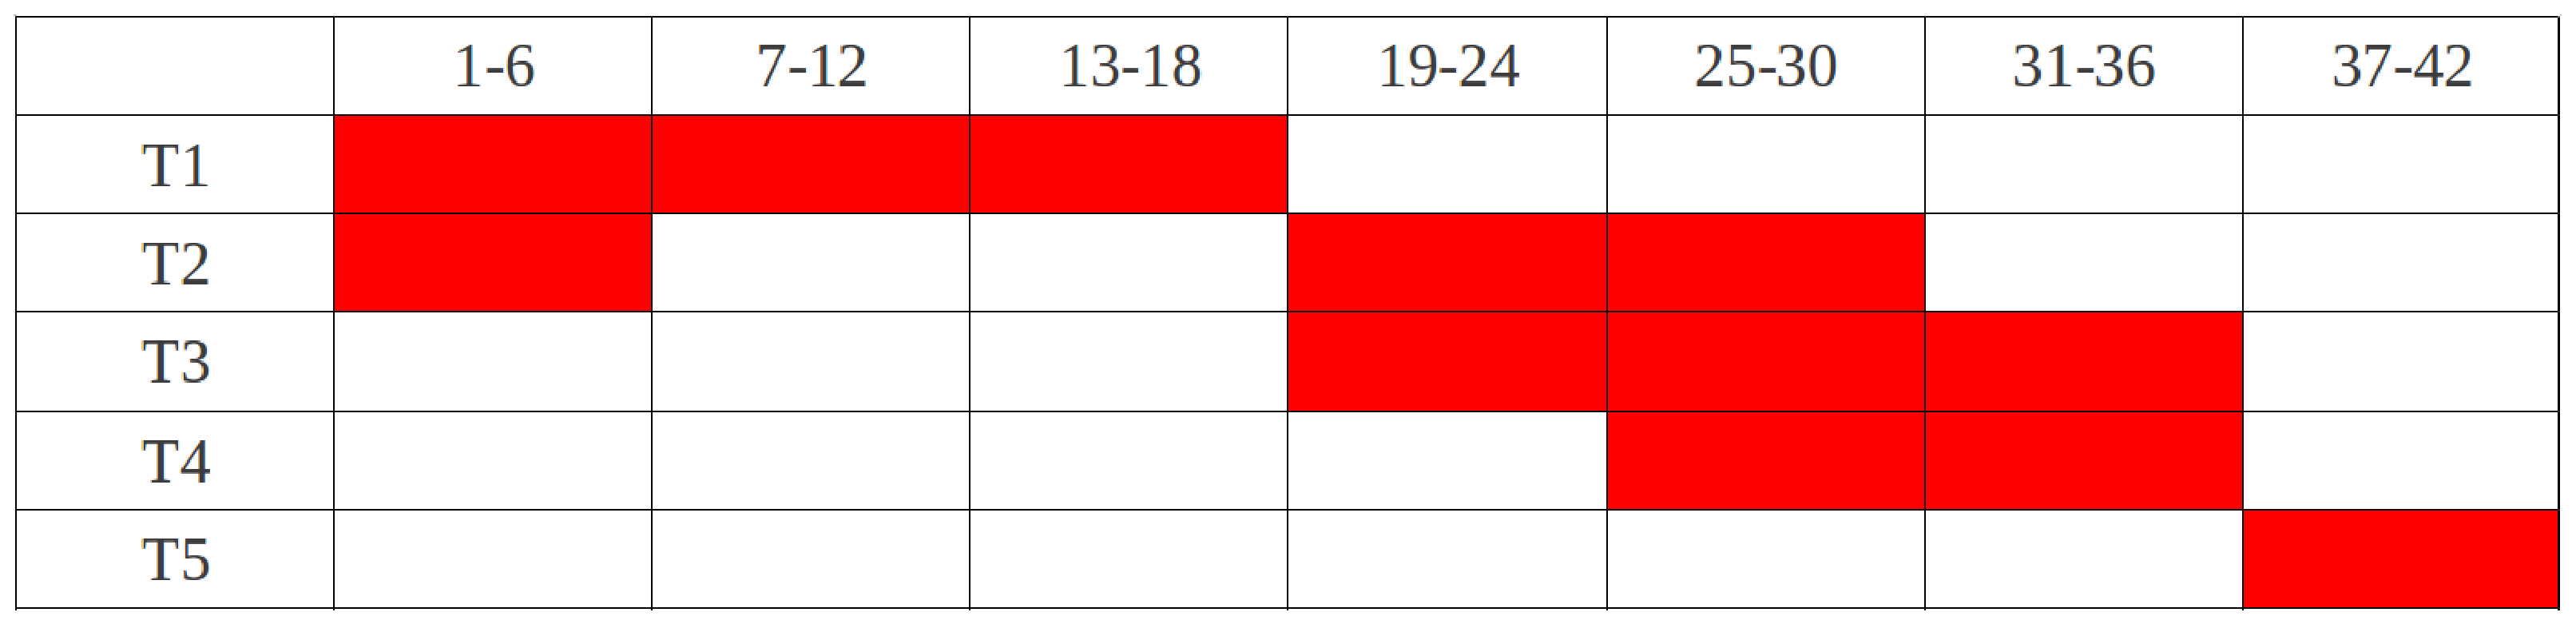
\includegraphics[width = 10cm]{planning.eps}
\caption{Planning of the different work packages, the columns represents the months.}
\label{fig:planning}
\end{figure}


\bibliographystyle{plainnat}
\bibliography{research-proposal}

\end{document}
